\chapter{Výběr algoritmu pro detekci pózy}
\label{sec:Pose}

Jelikož je dnes dostupných mnoho různých algoritmů či modelů pro detekci pózy
osob v obrázku či videu, nemá smysl pro naše řešení tvořit takovýto algoritmus
od nuly. Možné by to samozřejmě bylo, i vzhledem k dostupnosti otevřených
trénovacích dat (např. dataset COCO \cite{coco}), nicméně bychom pravděpodobně
nedosáhli kvalitních výsledků, jako řešení, která jsou výsledkem mnoholetých
výzkumů. Hlavně pak bychom těžko dosáhli výkonů těchto řešení, a ten je pro nás
stěžejní, jelikož potřebujeme video zpracovávat v reálném čase.

V následující kapitole budou popsány obecné principy detekce osob a jejich pózy
v obraze. Následně budou popsány některé populární algoritmy pro detekci pózy
se zaměřením na jejich specifika. Několik z nich pak bude otestováno, výsledky
budou porovnány, a na jejich základě bude zvolen algoritmus použitý v konečném
řešení detekce pádu.

\section{Detekce objektů a osob v obraze}

Detekce osob se v podstatě může generalizovat na detekci objektů v obraze.
Detekci objektů v obraze definujeme jako úlohu, kdy ve vstupním obrázku určíme
lokaci a třídu všech hledaných objektů.

V kapitole \ref{sec:CNN} jsme si popsali základní architekturu konvolučních
neuronových sítí, ta se ale většinou v praxi používá pro klasifikaci obrázků,
nikoliv pro detekci objektů - algoritmus tedy pouze určí, o jakou třídu objektu
se jedná, a ideálně potřebuje, aby objekt vyplňoval celý vstupní obraz.
Teoreticky by bylo možné detekci formulovat jako regresní problém a natrénovat
takovou síť, která by pomoci několika konvolučních vrstev následovaných
několika plně propojenými vrstvami byla schopna predikovat lokalizaci a třídu
všech objektů v obraze. \cite{szegedy} Problém detekce je ale velice komplexní
a taky by vyžadoval velice komplexní síť - více vrstev s mnoha filtry, resp.
neurony. Jak již ale bylo v zmiňováno, komplexnost sítě zvyšuje její nároky na
výpočetní výkon a komplikuje nebo úplně znemožňuje její trénování s ohledem na
pravděpodobnost přetrénování.

Snahou tedy je najít metody, které poupraví funkčnost sítě tak, aby byla
schopna efektivní detekce objektů. Většina těchto metod se nějakým způsobem
snaží rozdělit vstupní obrázek na menší části, ty následně jednak klasifikovat,
a tedy určit, zda se v dané lokalitě vyskytuje objekt, popřípadě pomocí regrese
určit jeho přesnou lokalizaci. Lokalizace je většinou reprezentována jako
souřadnice obdélníku ohraničujícího daný objekt, tzv. bounding box. Rozdělení
může být provedeno přímo na vstupním obrázku nebo na mapě příznaků v rámci
sítě. Taky můžeme buď rozdělit obrázek na pevně dané oblasti (např. do mřížky)
- jednofázový přístup, anebo v jedné fázi předpřípravit množinu oblastí a ve
druhé fázi nad těmito oblastmi provést klasifikaci a regresi - dvoufázový
přístup.

\subsection{Sliding window}

Jednou z prvních takových metod byl tzv. sliding window (klouzavé okno), který
aplikuje hrubou sílu. Vstupní obrázek se postupně projíždí oknem o fixní
velikosti. Vznikne tak množina pokrývající každou možnou lokaci objektů. Na
tyto oblasti se pak aplikuje klasifikační algoritmus. Postup se opakuje pro
několik velikostí okna, aby se detekovalo objekty různé velikosti.

Tento postup je ale velice pomalý, jelikož je pro každý obrázek zvolený velký
počet oblastí, pro které je třeba provést klasifikaci popřípadě regresi. Navíc
je většina těchto oblastí prázdná, a dochází tak k plýtvání výpočetním výkonem.
Algoritmus se taky potýká s překrývajícími se objekty.

Další metody se tedy snaží redukovat počet oblastí, na které se aplikuje
klasifikace, tak, že se vybere pouze oblasti, které pravděpodobně budou
obsahovat nějaký objekt.

\subsection{Dvoufázový přístup}

\subsubsection{R-CNN}
Prvním algoritmem, který efektivně zredukoval počet oblastí pro klasifikaci,
byl algoritmus R-CNN (Region-based Convolutional Network). \cite{r-cnn} Tento
algoritmus nejprve použil některou z dostupných metod (autoři použili selective
search) pro vygenerování navržených oblastí (region proposals), které
pravděpodobně obsahují nějaký objekt. Tyto metody jsou nezávislé na třídě
objektů. Algoritmus tedy vygeneruje zhruba 2000 oblastí, vzniklé obrázky jsou
následně upraveny na velikost požadovanou CNN v další fázi. CNN extrahuje z  
dané oblasti mapu příznaků, na její základě plně propojené vrstvy predikují
třídu objektu popřípadě jeho bounding box.

Problémem R-CNN je, že výběr oblasti a jejich následná klasifikace jsou
nezávislé úlohy a jsou nezávisle trénovány. Detekce objektu je taky poměrně
pomalá, protože je extrakce příznaků prováděná pro všechny oblasti zvlášť. Tyto
problémy se snaží řešit další upravené verze R-CNN.

\subsubsection{Fast R-CNN}
První z nich je Fast R-CNN \cite{fast-r-cnn}, která je upravená tak, aby bylo
možné provádět trénování v jednom kroku. Taky extrahuje příznaky pro celý
vstupní obraz najednou, pomocí selective search pak identifikuje oblasti zájmu
(RoI - Region of Interest), které následně použije pro klasifikaci a regresi.
Tato metoda je přesnější a asi desetkrát rychlejší než původní R-CNN.

\subsubsection{Faster R-CNN}
Další algoritmus, Faster R-CNN \cite{faster-r-cnn}, nahrazuje metodu selective
search vlastní, plně konvoluční sítí RPN (region proposal network).
Zefektivňuje tak proces trénování, výsledná síť je také rychlejší a přesnější
než Fast R-CNN.

\subsection{Jednofázový přístup}

Jednofázový přístup se snaží najít řešení, ve kterém není nutné hledat navržené
oblasti, ale provést klasifikaci a regresi na předem dané množině oblastí,
obvykle určené mřížkou.

\subsubsection{YOLO}
Prvním takovým algoritmem byl YOLO (taky YOLOv1, z ang. You Only Look Once)
\cite{yolo}. Ten, v původní verzi, rozdělí vstupní obraz do pevně dané mřížky
velikosti $S \times S$ a v každém z těchto polí určí $B$ bounding boxů a jejich
třídu. V původní verzi bylo zvoleno $S = 7$ a $B = 2$.

Obraz je nejprve zpracován pomocí konvolučních vrstev, které extrahují mapu
znaků o velikosti $S \times S \times K$, kde $K$ je počet kanálů. Každý pixel
této mapy představuje jedno pole mřížky. Dále je mapa zpracována plně
propojenými vrstvami, které provádějí nad každým polem mřížky klasifikaci a
regresi, viz obrázek \ref{fig:yolo}.

\begin{figure}[]
    \centering
    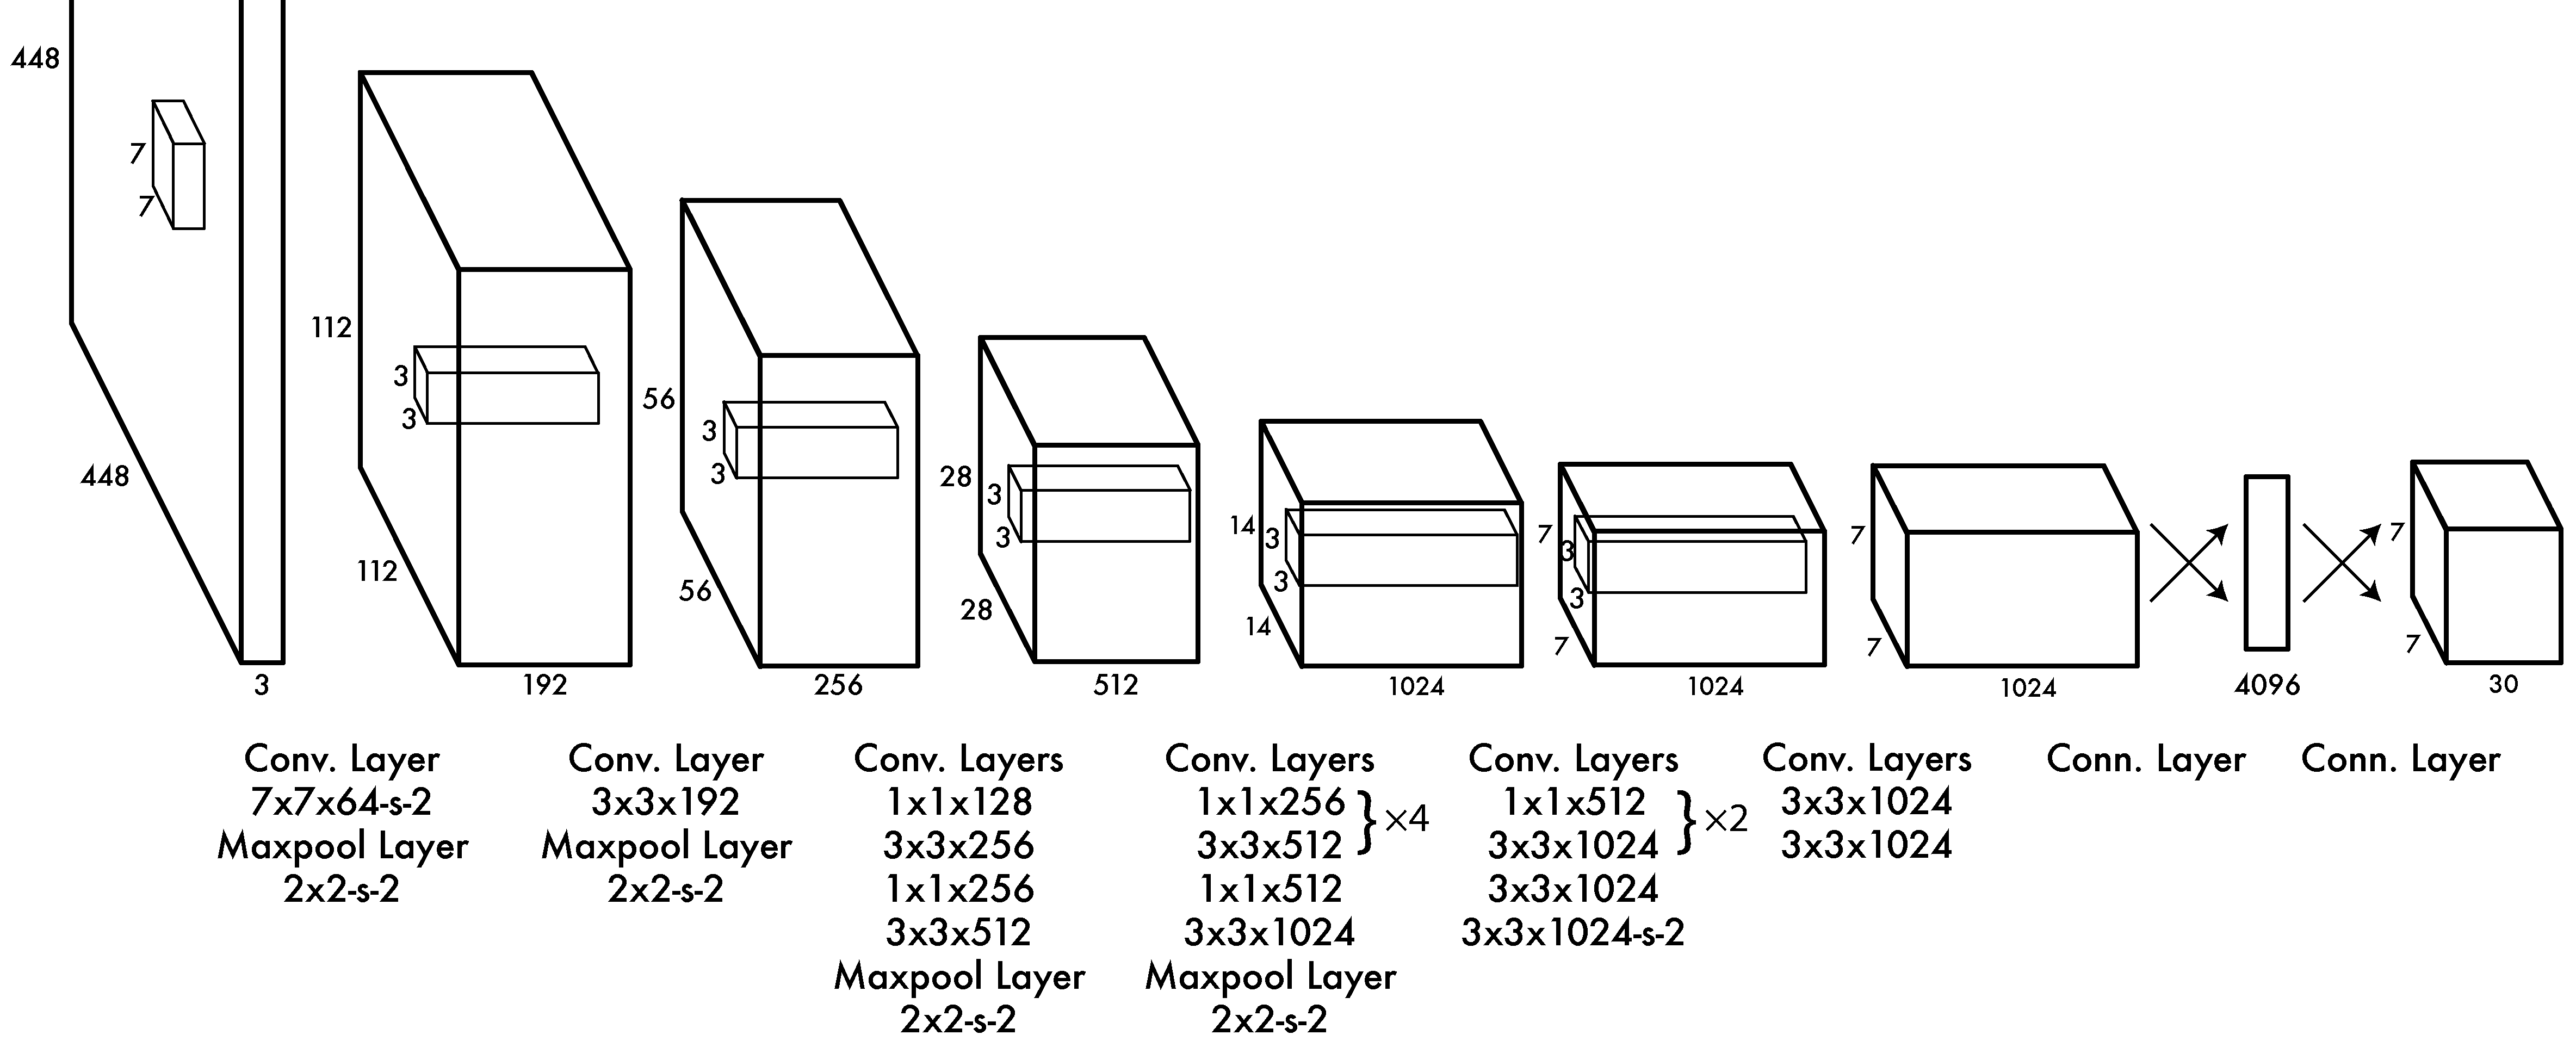
\includegraphics[width=\textwidth]{Figures/yolo}
    \caption{Architektura původní verze YOLO \cite{yolo}}
    \label{fig:yolo}
\end{figure}

Každý bounding box je reprezentován souřadnicemi středu a velikosti (šířka a
výška). Dohromady s informací o jistotě detekce bounding boxu (confidence
score) vrátí model $5$ informací o každém bounding boxu. Pro každé pole mřížky
pak určí společnou informaci o třídě všech objektů v daném poli. Pokud objekt
není detekován, třída indikuje pozadí a souřadnice bounding boxu jsou
ignorovány. Velikost výstupního vektoru je tedy $7 \times 7 \times (2 * 5 +
    C)$, kde $C$ je počet definovaných tříd - v původní verzi pouze 20.

Tento algoritmus, navržený v roce 2015 J. Redmonem et al., byl revolučně
rychlý, zároveň v porovnání s jinými real-time detekčními algoritmy dosahoval i
slušné přesnosti. Nicméně byl velice citlivý na velikost objektu a přesnost
detekce, zejména u menších objektů, byla horší než u dvoufázových algoritmů.

Další verze algoritmu YOLO přinesly postupná vylepšení ve formě optimalizace
trénování a architektury. YOLOv2 \cite{yolo9000} zavedl mj. trénování na
několika měřítkách a byl natrénován s 9000 třídami (proto taky nazýván
YOLO9000). YOLOv3 \cite{yolov3} přinesl mj. detekci na několika měřítkách.
Postupně byla taky zvětšována mřížka a měnila se použitá architektura CNN sítě
sloužící pro extrakci příznaků pro jednotlivá pole mřížky. Postupně taky byly
přidávány další funkce jako je segmentace, detekce pózy či sledování objektů
(ang. tracking).

V 2020 roce firma Ultralytics poprvé implementovala YOLO s využitím populární
knihovny PyTorch (YOLOv5), což umožnilo snadnější využití YOLO v praxi. Firma
Ultralytics také vytvořila framework pro použití různých verzí YOLO (YOLOv3 a
novější). Také pracuje na dalších vylepšeních a optimalizacích. Konkrétně
vytvořila YOLOv5 (2020), YOLOv8 (2023) a YOLOv11 (2024).

\subsubsection{SSD}
Dalším populárním algoritmem, který používá jednofázový přístup, je SSD (z ang.
single shot detector). \cite{szegedy:ssd}

\begin{figure}[]
    \centering
    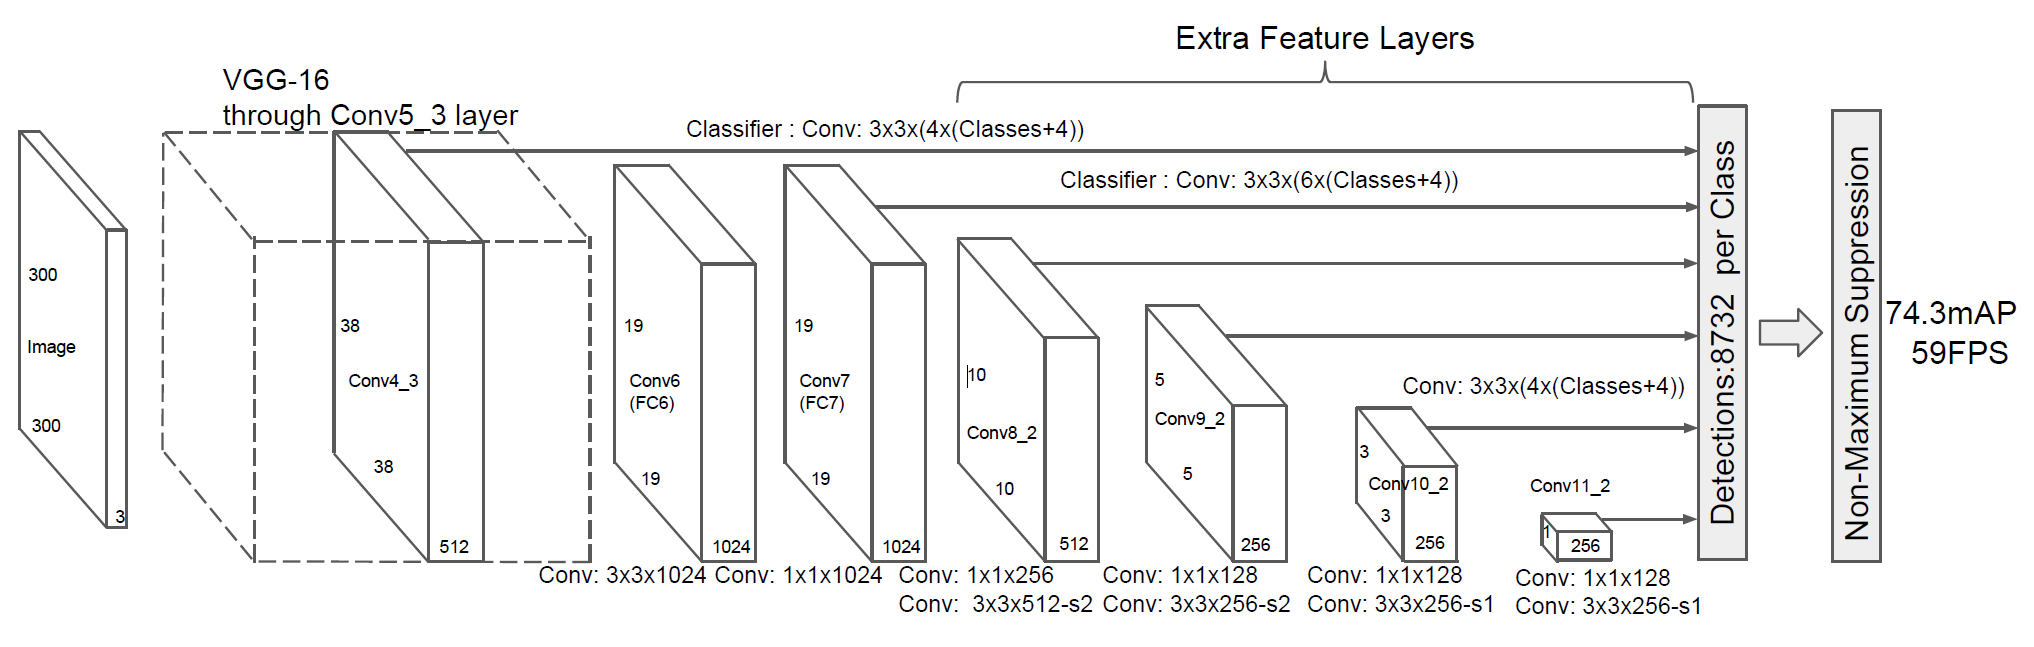
\includegraphics[width=\textwidth]{Figures/ssd.png}
    \caption{Architektura SSD \cite{szegedy:ssd}}
    \label{fig:ssd}
\end{figure}

% openpifpaf, mediapipe(shufflenet, resnet), torchvision, yolo

\endinput